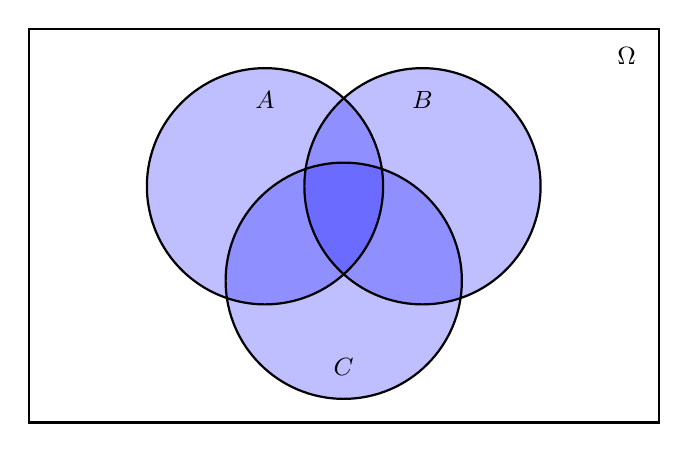
\begin{tikzpicture}[font=\small]
  % Parameters
  \def\W{8}   % rectangle width
  \def\H{5}   % rectangle height
  \def\r{1.5} % circle radius

  % Rectangle (sample space)
  \draw[thick] (0,0) rectangle (\W,\H) node[pos=0.98,below left] {$\Omega$};

  % Clip everything to the rectangle so circles stay inside
  \begin{scope}
    \clip (0,0) rectangle (\W,\H);

    % Fill the union by filling each circle with same color and opacity
    \fill[blue,opacity=0.25] (3.0,3.0) circle (\r); % A
    \fill[blue,opacity=0.25] (5.0,3.0) circle (\r); % B
    \fill[blue,opacity=0.25] (4.0,1.8) circle (\r); % C
  \end{scope}

  % Draw circle outlines and labels
  \draw[thick] (3.0,3.0) circle (\r) node[yshift=1.1cm] {$A$};
  \draw[thick] (5.0,3.0) circle (\r) node[yshift=1.1cm] {$B$};
  \draw[thick] (4.0,1.8) circle (\r) node[yshift=-1.1cm] {$C$};

  % Title / probability text
  %\node at (4,-0.5) {$P(A\cup B\cup C)$};

\end{tikzpicture}